The same analysis staregy is used to derive upper limits on the $S_{8}S_{8}\rightarrow t\bar{t}t\bar{t}$ production cross section. The limits are first extarcted from 1L/2LOS and 2LSS/ML final staes individually. 
For the mass points with $m_{S_8} \leq 1$~\TeV, the $m_{H/A}$-parametrised MVAs (GNN for 1L/2LOS and BDT for 2LSS/ML) are evaluated at $m_{S_8} = m_{H/A}$.
At each mass point, the binning of the fitted distributions is the same as the one used for $H/A$. For $m_{S_8} > 1$~\TeV, the GNN/BDT and binning for $m_{H/A} = 1$~\TeV\ are adopted.
The 95\% CL upper limits on the $S_{8}S_{8}\rightarrow t\bar{t}t\bar{t}$ production cross section of the two individual fianl states are shown in Figure \ref{fig:sgluon_individual}.

\begin{figure}[htbp!]
    \centering
    \begin{subfigure}[t]{0.49\textwidth}
      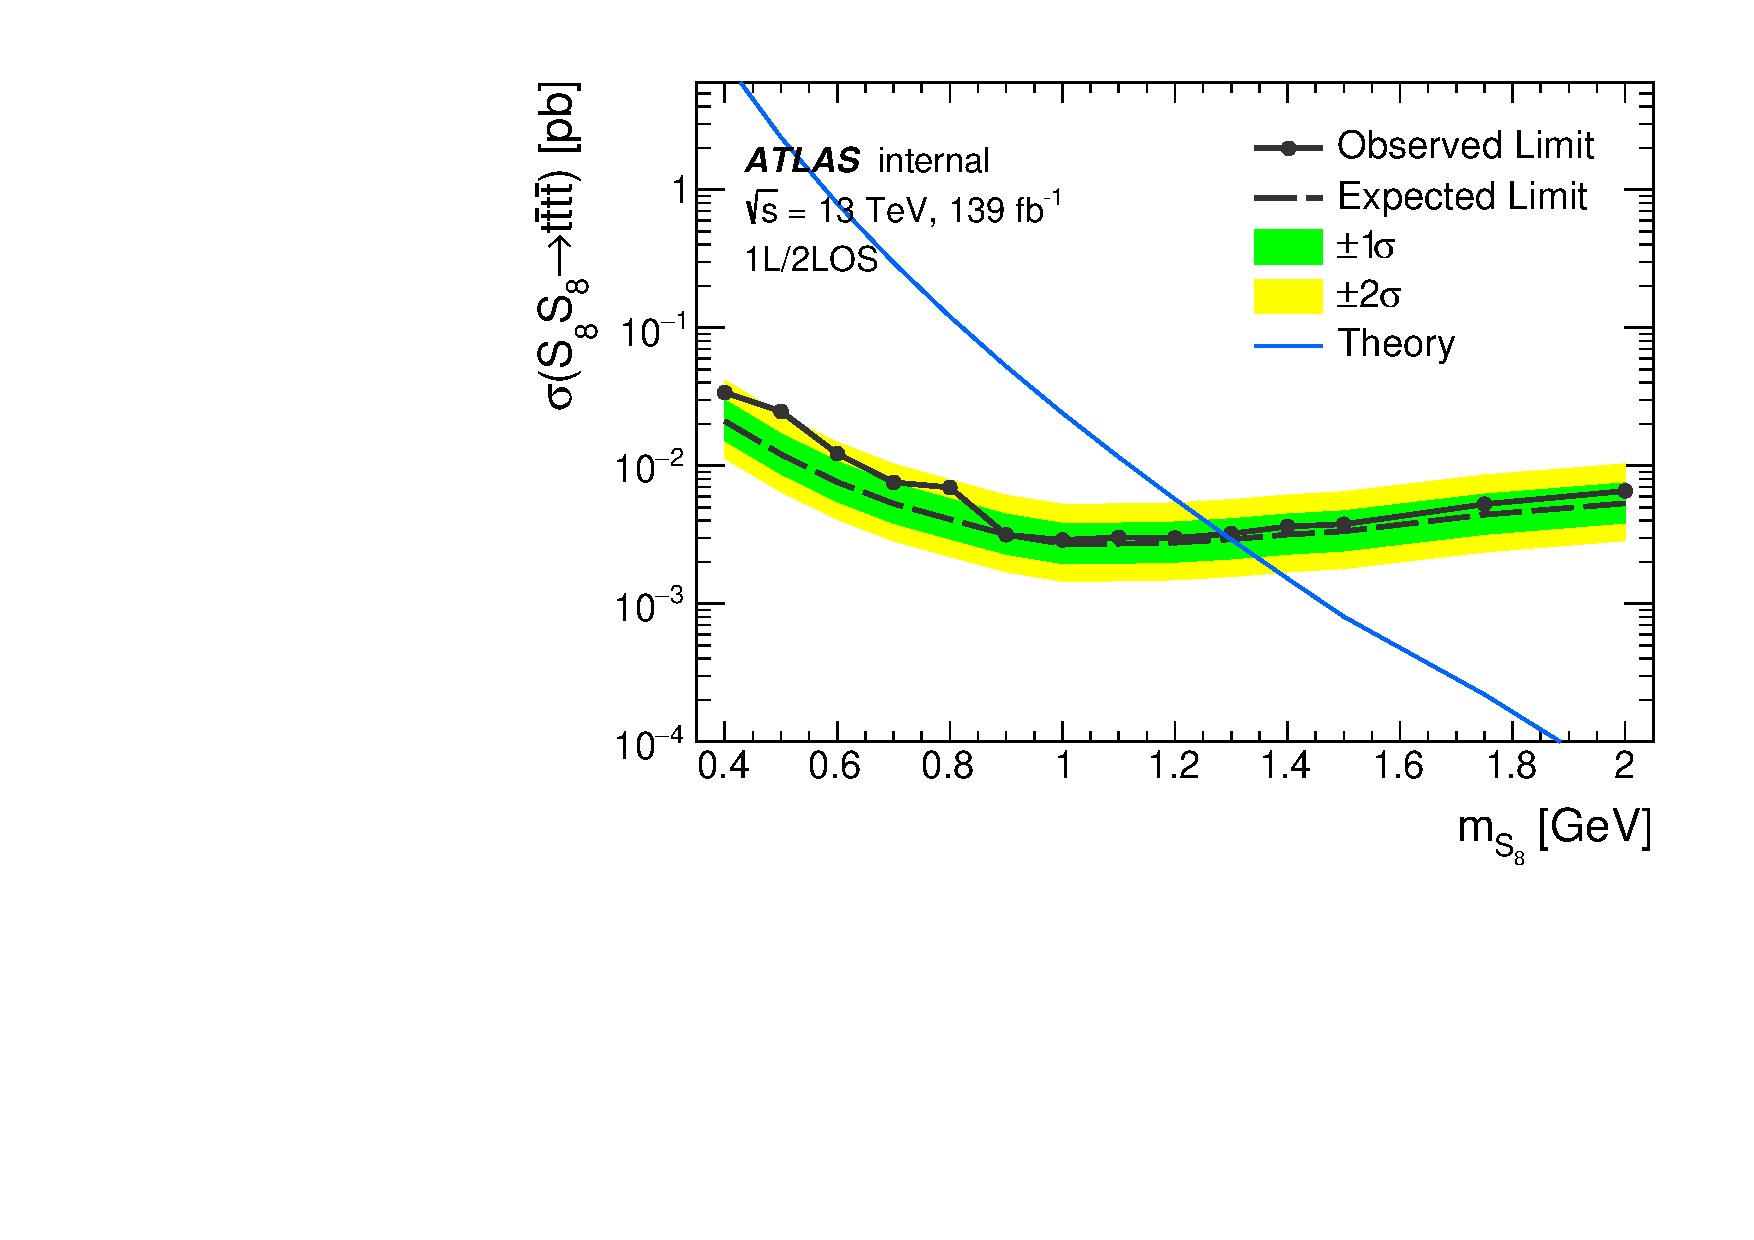
\includegraphics[width=1 \textwidth]{figures/sgluon_limits/lim_1LOS.pdf}
      \caption{1L/2LOS}
    \end{subfigure}
    \begin{subfigure}[t]{0.49\textwidth}
      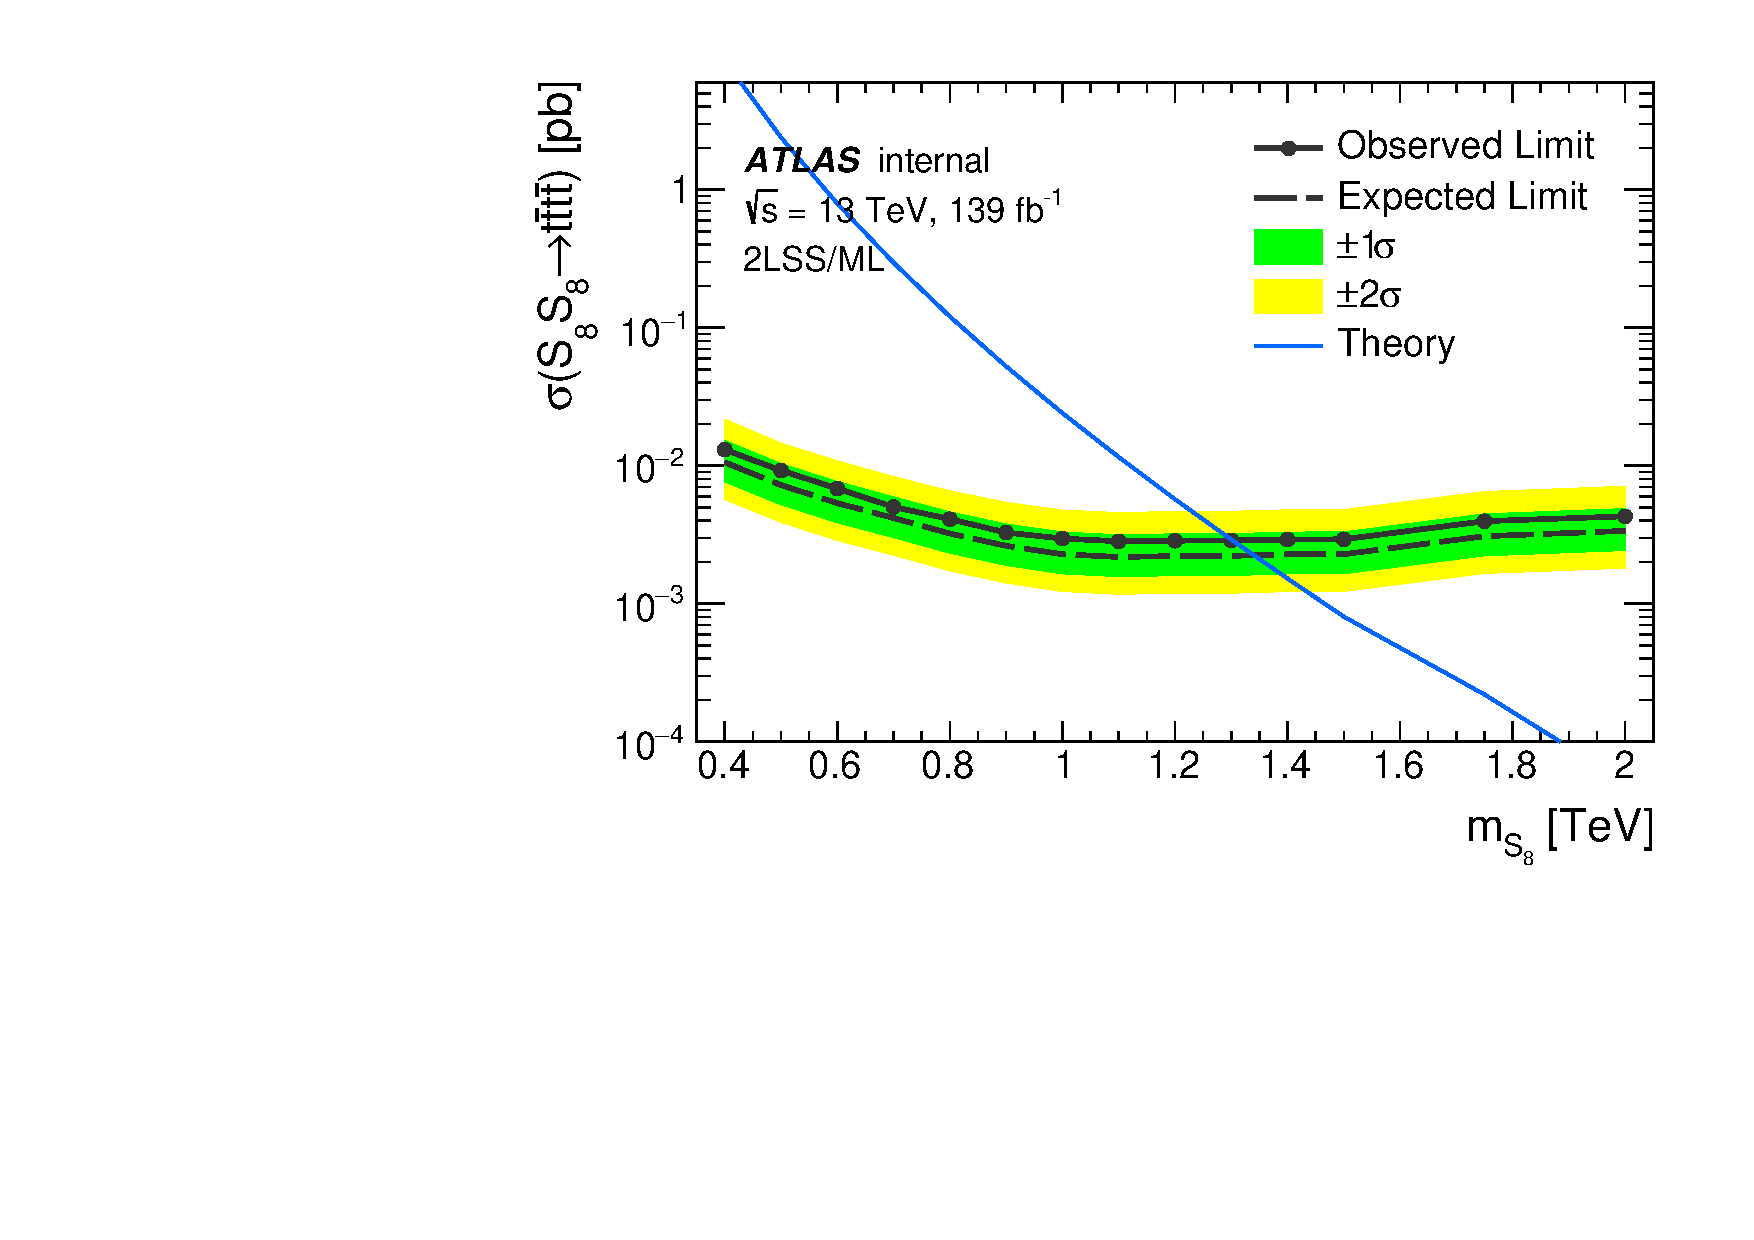
\includegraphics[width=1 \textwidth]{figures/sgluon_limits/lim_SSML.pdf}
      \caption{2LSS/ML}
    \end{subfigure}
    \caption{\label{fig:sgluon_individual}Observed and expected 95\% CL upper limit on the cross section for the production of $S_{8}S_{8}\rightarrow t\bar{t}t\bar{t}$ as a function of $m_{S_{8}}$ in 1L/2LOS (left) and 2LSS/ML (right) final states.}
\end{figure}

The 1L/2LOS and 2LSS/ML final states are combined to determine the final limits. The resulting 95\% CL upper limits on the $S_{8}S_{8}\rightarrow t\bar{t}t\bar{t}$ production cross section are illustrated in Figure \ref{fig:sgluon_combination}. 
The observed and expected upper limits from the combination of 1L/2LOS and 2LSS/ML final states are shown, compared to the expected limits from using only the 1L/2LOS or the 2LSS/ML final states. 
The behaviour of the limits for $m_{s_{8}} \leq 1$~\TeV\ is similar to that for $t\bar{t}H/A \rightarrow t\bar{t}t\bar{t}$ production, with an improvement of up to 26\% when using the combination with respect to using the 2LSS/ML final states only. 
The limits slightly weaken for $m_{s_{8}}>1$~\TeV\ given that the MVAs are optimised for $m_{H/A}=1$~\TeV\. Sgluon masses $m_{S_8} \leq 1.5$~\TeV\ are excluded at 95\% CL.

\begin{figure}[htbp!]
    \centering
    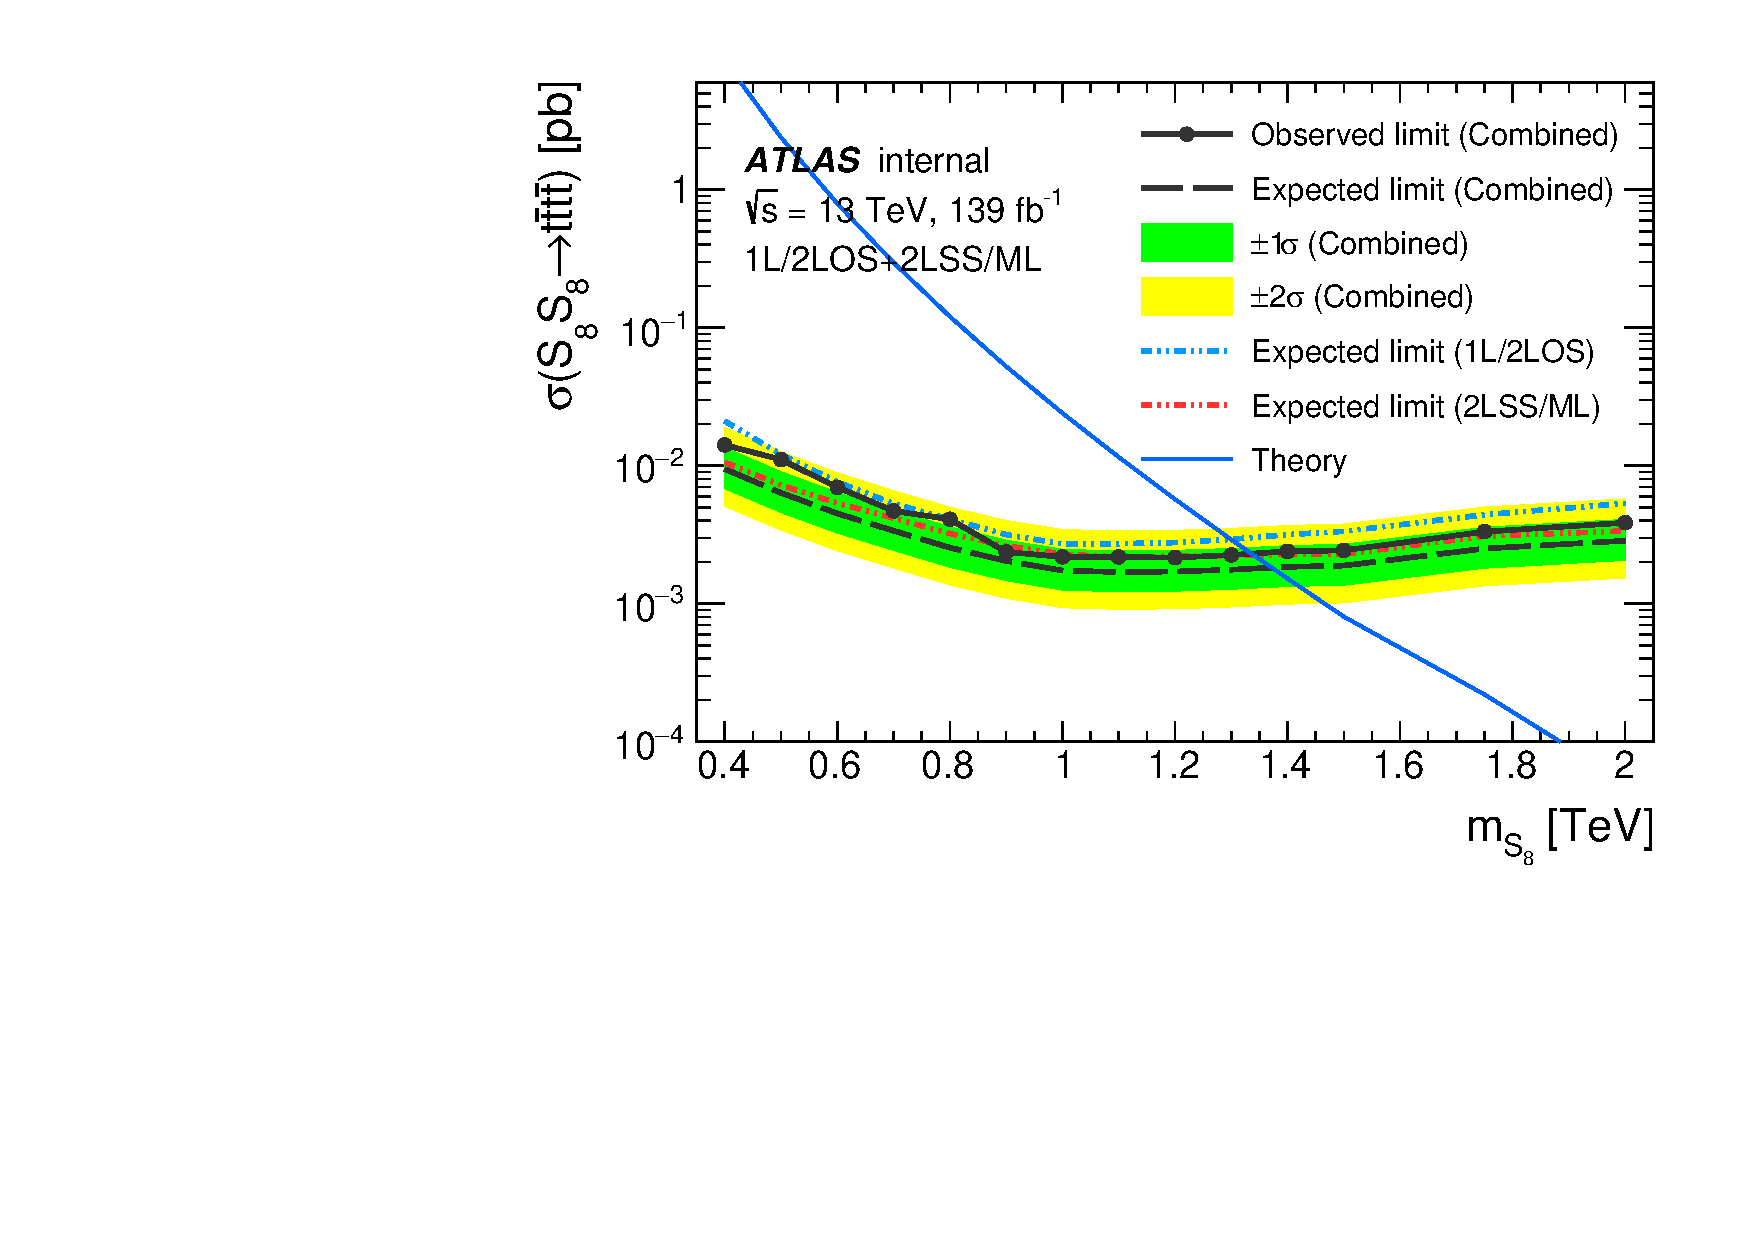
\includegraphics[width=0.49 \textwidth]{figures/sgluon_limits/lim_combined_with_individual_exp.pdf}
    \caption{\label{fig:sgluon_combination}Expected and observed 95\% CL upper limits
    on the $S_8S_8\rightarrow\tttt$ production cross section
    as a function of $m_{S_8}$,
    obtained from the combination of the 1L/2LOS and 2LSS/ML final states.
    The expected limits from the individual 1L/2LOS and 2LSS/ML analyses are also shown.
    The predicted production cross section from Ref.~\cite{Darm__2021} is shown with the solid blue curve.
    }
\end{figure}